\section{PROJECT BACKGROUND}

\subsection{Background}

\subsection{Background}

\begin{frame}[t]{Background}
    \footnotesize

    \begin{columns}[T,onlytextwidth]

        % =========================
        % Left: Message
        % =========================
        \column{0.42\textwidth}

        \textbf{Motivation}
        \vspace{0.12cm}

        \begin{itemize}
            \setlength\itemsep{0.18cm}
            \item Machine learning is widely used for classification and regression tasks.
            \item Many traditional models learn a \textbf{single global pattern} from the full dataset.
            \item However, real-world data may contain \textbf{heterogeneous subgroups} with different local behaviors.
            \item As a result, one global model may not capture all local patterns effectively.
            \item This motivates the need for \textbf{clusterwise learning}.
        \end{itemize}

        \vspace{0.18cm}

        % =========================
        % Right: Conceptual diagram
        % =========================
        \column{0.56\textwidth}

        \centering
        \resizebox{\linewidth}{!}{
            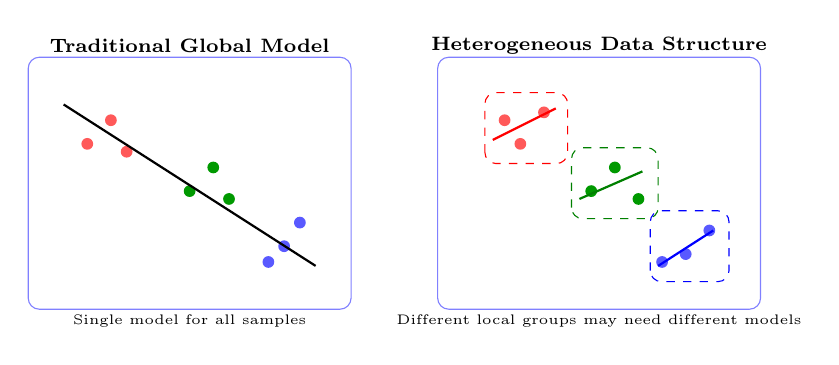
\begin{tikzpicture}[
                    font=\scriptsize,
                    panel/.style={draw=blue!50, rounded corners=4pt, minimum width=4.1cm, minimum height=3.2cm},
                    title/.style={font=\scriptsize\bfseries},
                    global/.style={thick, black},
                    locala/.style={thick, red},
                    localb/.style={thick, green!50!black},
                    localc/.style={thick, blue},
                    ptA/.style={circle, fill=red!65, inner sep=1.5pt},
                    ptB/.style={circle, fill=green!60!black, inner sep=1.5pt},
                    ptC/.style={circle, fill=blue!65, inner sep=1.5pt}
                ]

                % Panel 1
                \node[panel] (p1) at (0,0) {};
                \node[title] at (0,1.75) {Traditional Global Model};

                % points
                \node[ptA] at (-1.3,0.5) {};
                \node[ptA] at (-1.0,0.8) {};
                \node[ptA] at (-0.8,0.4) {};

                \node[ptB] at (0.0,-0.1) {};
                \node[ptB] at (0.3,0.2) {};
                \node[ptB] at (0.5,-0.2) {};

                \node[ptC] at (1.2,-0.8) {};
                \node[ptC] at (1.4,-0.5) {};
                \node[ptC] at (1.0,-1.0) {};

                % one global fit
                \draw[global] (-1.6,1.0) -- (1.6,-1.05);
                \node[font=\tiny] at (0,-1.75) {Single model for all samples};

                % Panel 2
                \node[panel] (p2) at (5.2,0) {};
                \node[title] at (5.2,1.75) {Heterogeneous Data Structure};

                % cluster A
                \node[ptA] at (4.0,0.8) {};
                \node[ptA] at (4.2,0.5) {};
                \node[ptA] at (4.5,0.9) {};
                \draw[red,dashed,rounded corners] (3.75,0.25) rectangle (4.8,1.15);

                % cluster B
                \node[ptB] at (5.1,-0.1) {};
                \node[ptB] at (5.4,0.2) {};
                \node[ptB] at (5.7,-0.2) {};
                \draw[green!50!black,dashed,rounded corners] (4.85,-0.45) rectangle (5.95,0.45);

                % cluster C
                \node[ptC] at (6.3,-0.9) {};
                \node[ptC] at (6.6,-0.6) {};
                \node[ptC] at (6.0,-1.0) {};
                \draw[blue,dashed,rounded corners] (5.85,-1.25) rectangle (6.85,-0.35);

                % local patterns
                \draw[locala] (3.85,0.55) -- (4.65,0.95);
                \draw[localb] (4.95,-0.20) -- (5.75,0.15);
                \draw[localc] (5.95,-1.05) -- (6.65,-0.60);

                \node[font=\tiny] at (5.2,-1.75) {Different local groups may need different models};

            \end{tikzpicture}
        }
    \end{columns}

    {\scriptsize
        \textbf{Transition:} This motivation leads to the development of \textbf{KFCProcedure} \cite{has2021kfc}.
    }

\end{frame}

\begin{frame}[t]{KFCProcedure Algorithm Workflow}
    \footnotesize
    \centering

    {\scriptsize
        \textbf{Clusterwise learning framework based on KFCProcedure}
        \cite{has2021kfc}
    }

    \vspace{0.18cm}

    \resizebox{0.93\linewidth}{!}{
        \begin{tikzpicture}[
                font=\scriptsize,
                box/.style={
                        draw=blue!60,
                        fill=lightblue,
                        rounded corners=4pt,
                        minimum width=1.35cm,
                        minimum height=0.65cm,
                        align=center
                    },
                widebox/.style={
                        draw=blue!60,
                        fill=lightblue,
                        rounded corners=4pt,
                        minimum width=2.45cm,
                        minimum height=0.65cm,
                        align=center
                    },
                aggbox/.style={
                        draw=blue!60,
                        fill=green!12,
                        rounded corners=4pt,
                        minimum width=3.9cm,
                        minimum height=0.8cm,
                        align=center
                    },
                note/.style={
                        anchor=west,
                        align=left,
                        text width=2.75cm,
                        font=\scriptsize
                    },
                arrow/.style={-Latex, thick},
                dashline/.style={dash pattern=on 5pt off 4pt, thick}
            ]

            % =========================
            % Step labels
            % =========================
            \node[anchor=east] at (-1.0,2.6) {\textbf{K-step}};
            \node[anchor=east] at (-1.0,1.25) {\textbf{F-step}};
            \node[anchor=east] at (-1.0,-0.25) {\textbf{C-step}};

            % =========================
            % K-step
            % =========================
            \node[box] (b1) at (0.8,2.6) {$\mathcal{B}_1$};
            \node[box] (b2) at (3.6,2.6) {$\mathcal{B}_2$};
            \node[box] (bm) at (6.6,2.6) {$\mathcal{B}_M$};
            \draw[dashline] (b2.east) -- (bm.west);

            \node[note] at (7.85,2.6) {
                Identifies hidden local structures in heterogeneous data.
            };

            % =========================
            % F-step
            % =========================
            \node[widebox] (m1) at (0.8,1.25) {$\mathcal{M}_{1,1}, \ldots, \mathcal{M}_{1,K}$};
            \node[widebox] (m2) at (3.6,1.25) {$\mathcal{M}_{2,1}, \ldots, \mathcal{M}_{2,K}$};
            \node[widebox] (mm) at (6.6,1.25) {$\mathcal{M}_{M,1}, \ldots, \mathcal{M}_{M,K}$};
            \draw[dashline] (m2.east) -- (mm.west);

            \node[note] at (7.85,1.25) {
                Trains supervised models for each discovered local group.
            };

            % =========================
            % C-step
            % =========================
            \node[aggbox] (agg) at (3.6,-0.25) {COBRA-Based\\Aggregation};

            \node[note] at (7.85,-0.25) {
                Combines local model predictions into the final output.
            };

            % =========================
            % Arrows
            % =========================
            \draw[arrow] (b1.south) -- (m1.north);
            \draw[arrow] (b2.south) -- (m2.north);
            \draw[arrow] (bm.south) -- (mm.north);

            \draw[arrow] (m1.south east) -- (agg.north);
            \draw[arrow] (m2.south) -- (agg.north);
            \draw[arrow] (mm.south west) -- (agg.north);

        \end{tikzpicture}
    }

    \vspace{0.45cm}

    {\scriptsize
        \textbf{Key idea:} KFCProcedure provides the clusterwise workflow, while COBRA provides the reusable combiner for the C-step.
    }

\end{frame}


\subsection{Problem Statement}

\begin{frame}[t]{Problem Statement}
    \footnotesize
    \begin{itemize}
        \setlength\itemsep{0.22cm}

        \item \textbf{Lack of unified architecture for aggregation methods}

              Different aggregation strategies such as averaging, voting, and COBRA-based methods need a consistent structure for implementation and comparison.

        \item \textbf{Limited modularity and extensibility}

              Without a reusable package design, adding new base estimators, clustering methods, or combiner strategies becomes difficult and less maintainable.
    \end{itemize}

    \vspace{0.18cm}

    \begin{block}{Engineering Need}
        A modular machine learning package is needed to support clusterwise learning, local model training, and flexible prediction aggregation.
    \end{block}

\end{frame}

\subsection{Objective}

\begin{frame}[t]{Objective}
    \footnotesize

    \begin{itemize}
        \setlength\itemsep{0.24cm}

        \item To study and implement the theoretical foundations of
              \textbf{KFCProcedure} and \textbf{COBRA-based aggregation methods}.

        \item To develop \textbf{KFCProcedure} as a clusterwise learning framework
              based on the K-step, F-step, and C-step workflow.

        \item To redesign \textbf{GradientCOBRA} as a reusable combiner architecture
              that supports flexible aggregation strategies for the C-step.

        \item To build a modular Python package with clear documentation, practical examples,
              and a consistent API for researchers and practitioners.
    \end{itemize}

\end{frame}


